
\subsubsection*{Условие квазистационарности}
Условие квазистационарности заключается в том, что характерное время изменения макроскопических величин (таких как ток, напряжение, частота или импеданс) в цепи должно быть сильно меньшим времени распространения сигнала в цепи (размер цепи делить на скорость света).


\subsubsection*{Зарядка и разядка конденсатора}

% \begin{figure}[h]
%     \centering
%     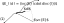
\includegraphics[width=0.3\textwidth]{img/2.jpg}
%     %\caption{}
%     %\label{fig:}
% \end{figure}

Зарядка и разрядка конденсатора описывается следующим дифференциальным уравнением и его решением ($U_c$ -- напряжение на конденсаторе): 
$$
    E = U_c + RC\dot{U_c};
    \hspace{0.5cm} 
    U_c = E - ke^{-RCt}
$$ \text{где} $k$ - постоянная интегрирования, зависит от начального напряжения на конденсаторе, а $RC$ - характерное время зарядки конденсатора.


\subsubsection*{Установлени тока в катушке индуктивности}

Если в схеме для конденсатора заменить его на индуктивность, то получим следующее уравнение и его решение ($k$ - постоянная интегрирования, зависящая от начального тока): 
$$
    E = IR + \dot{I}L; \hspace{0.5cm} 
    I = \frac{E}{R} + ke^{-\frac{R}{L}t}; \hspace{0.5cm} 
    k = I_{\text{нач}} - \frac{E}{R}
$$


\subsubsection*{Интегрирующие и дифференцирующие цепочки}

\begin{figure}[h]
    \centering
    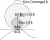
\includegraphics[width=0.5\textwidth]{img/1.jpg}
    %\caption{}
    %\label{fig:}
\end{figure}


Если в нарисованной выше схеме подавать вместо $E$ какой-то сигнал, то в случае а):
$$
    E(t) = U_c + \dot{U_c}CR \approx \dot{U_c}R;\
    \hspace{0.5cm} 
    U_c \approx \frac{1}{RC}\int E(t)dt,
$$
В случае б):
$$
    E(t) = U_c + \dot{U_c}CR \approx U_c;
    \hspace{0.5cm}  U_R \approx RC\frac{dE(t)}{dt}.
$$



\subsubsection*{Свободные колебания в линейных системах. Колебательный RLC-контур.}
\includegraphics[scale=0.34]{img/RLCcircuit1.png}
\newline
Если контур состоит из последовательно стоящих резистора, конденсатора и индуктивности то процессы в нём описываются дифференциальным уравнением 
$$
    U_c + \dot{U_c}RC + \ddot{U_c}CL = 0\Leftrightarrow\ddot{U_c} + \dot{U_c}\frac{R}{L} + \frac{U_c}{LC} = 0\Leftrightarrow\ddot{U_c} + 2\gamma\dot{U_c} + \omega_0^2U_c = 0;\;\;\;\text{где}\;\gamma = \frac{R}{2L},\;\omega_0 = 1/\sqrt{LC}
$$
Решением будет $U_c(t) = A_1e^{(-\gamma-\sqrt{\gamma^2-\omega_0^2})t}+A_2e^{(-\gamma+\sqrt{\gamma^2-\omega_0^2})t}$, $(A_1 + A_2 = U_c(0);\; C\dot{U_c}(t) = I(0))$. \newline Для тока уравнение и решение точно такое же, а коэффициенты находятся из $A_1 + A_2 = I(0);\newline I(0)R + U_c(0) + L\dot{I}(0) = 0$.
\newline
\textbf{Если} $\omega_0 > \gamma$, то можно сразу найти синусоидальное (периодическое) решение:
$$U_c(t) = B_1e^{-\gamma t}cos(\omega t - \theta_1);\;\;I(t) = -B_2e^{-\gamma t}\cos(\omega t - \theta_2);\;\;\text{где}\;\omega = \sqrt{\omega_0^2 - \gamma^2}$$
При условии $U_c(0) = U_0;\;I(0) = 0;$ получаем: $\theta_2 = \frac{\pi}{2}; B_2 = \frac{U_0}{L\omega}; \theta_1 = -arctan(\gamma/\omega); B_1 = U_0\omega_0/\omega$
\newline Коэффициент $\frac{U_0}{L\omega}$ можно найти из уравнения: $\frac{dI}{dt}(0)L + I(0)R + U_0 = 0$ \newline
\textbf{Если} $\omega_0 \leqslant \gamma$, то решение называется апериодическим:
$$U_c = U_0e^{-\gamma t}(\frac{\gamma}{\varkappa}sh\varkappa t+ch\varkappa t);\;I = -\frac{U_0}{L\varkappa}e^{-\gamma t}sh\varkappa t;\;\text{где}\;\varkappa = i\sqrt{\omega_0^2 - \gamma^2} = i\omega$$
\begin{center}
\includegraphics[scale=0.3]{img/RLCcircuit2.png}
\end{center}
$R = 2\sqrt{L/C}$ и сам процесс, соответствующий режиму $\omega_0 = \gamma$ называют критическими:
$$
    \text{Предельным\;переходом\;из\;прошлого\; выражения: }
    I = -\frac{U_0}{L}te^{-\gamma t};\;U_c = U_0e^{-\gamma t}(1+\gamma t)
$$
\subsubsection*{Коэффициент затухания, логарифмический декремент и добротность. Энергетический смысл добротности.}
Добротность называют величину: $Q = 2\pi\frac{W}{\Delta W}$, \text{где} $W$ - энергия в контуре в какой-то момент времени, $\Delta W$ - потери в контуре за период. Будем рассматривать добротность только при слабом затухании $\gamma \ll \omega_0$.
$$
    U_c \approx U_0e^{-\gamma t}cos\omega_0 t;\;W = \frac{CU^2}{2} = CU_0^2e^{-2\gamma t}\text{\;(удобнее\; рассматривать\;моменты\;когда\;}I = 0)
$$
Потеря энергии за период равна (учтём что $\gamma \ll \omega_0;\;\text{или}\;2\gamma T \ll 1)$
$$
    \Delta W = \frac{CU_0^2}{2}(e^{-2\gamma t} - e^{-2\gamma(t+T)}) = W(1-e^{-2\gamma T}) \approx 2\gamma TW
$$
$$
    Q = 2\pi \frac{W}{\Delta W} = \frac{\pi}{\gamma T} \approx \frac{1}{R}\sqrt{\frac{L}{C}}
$$
Логарифмическим коэффициентом затухания $\theta$ называется логарифм отношения двух последовательных максимальных отклонений в одну сторону.
$$
    \theta = ln\frac{U_k}{U_{k+1}} = lne^{\gamma T} = \gamma T = \frac{\pi}{Q}
$$
